\chapter{Referencial Teórico}

\section{Iluminação de LED}

\subsection{LED}

O \acf{LED} mudou a forma como a humanidade gera luz. Atualmente são usados em inúmeras aplicações indicativas, iluminação, TVs e vários outros usos. O processo de emissão de luz por um material de estado-sólido estimulado por uma fonte de energia elétrica, denominado de eletroluminescência, foi primeiramente observado em 1907 por Henry Joseph Round (1881-1966) \cite{led}, quando investigava o uso de cristais de carbeto de silício (SiC conhecido também como \textit{corborundum}) como "cristais retificadores" responsáveis por demodular sinais modulados em amplitude nos rádios da época. A junção responsável pelo contato destes cristais e alguns metais (junção característica de diodos \textit{Schottky}) vinha sendo testada como possível substituta aos caros e ineficientes tubos de vácuo eletrônicos (ou válvulas termiônicas). Henry observou que alguns pontos do cristais brilhavam ao aplicar-se potenciais, na faixa de 10 a 110 V, com os contatos metálicos.

As primeiras investigações detalhadas sobre eletroluminescência foram feitas pelo inventor russo Oleg Vladimirovich Losev (1903-1942) que publicou seu primeiro artigo aos 20 anos em 1923, ainda sem educação formal, e reportou observar luz verde ao polarizar reversamente um retificador de junção metal-cristal de SiC. Losev também observou corretamente que a razão do fenômeno não tinha relação com incandescência pois ocorria a temperatura ambiente. Mais tarde, em 1933, Losev também estudou o efeito da eletroluminescência em junções semicondutoras "p-n" com destaque para suas observações quanto à relação entre a energia emitida pelo diodo e a energia de "\textit{gap}" do material.

Eletroluminescência é definida como a emissão de luz por um material semicondutor quando exposto a um campo elétrico. Um junção P-N, quando polarizada diretamente, conduz corrente elétrica pois ocorre um fluxo de elétrons da região de semicondutor tipo N para a região tipo P e consequentemente, um fluxo de "buracos", portadores fictícios de carga positiva, no sentido oposto. Os elétrons e buracos se recombinam e neste processo energia é liberada, pois os primeiros se encontram na camada de condução no semicondutor tipo N e os buracos, na camada de valência do semicondutor tipo P.

\begin{figure}[ht]
    \begin{center}
    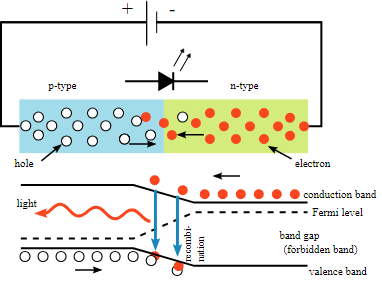
\includegraphics{figuras/led.PNG}
    \end{center}
    \caption[Diagrama de funcionamento do LED.]{Diagrama de funcionamento do LED. Acima, o esquema da junção p-n com o estímulo elétrico e abaixo o diagrama de banda de energia do semicondutor}
    \label{led}
\end{figure}

%By User:S-kei - File:PnJunction-LED-E.PNG, CC BY-SA 2.5, https://commons.wikimedia.org/w/index.php?curid=14985902 

A recombinação dos pares elétron-buraco libera energia pelo fato dos elétrons passarem para um nível menos energético \cite{rezende}. Uma vasta gama de materiais semicondutores apresenta uma estrutura de bandas de energia chamada de banda de "gap" indireto, e isso significa em resumo que a transição de elétrons entre os níveis energéticos não envolve apenas emissão ou absorção de luz (fótons), envolve também energia vibratória que gera calor (fônons). Alguns outros materiais têm o que se chama de banda de "gap" direta e a emissão de luz no caso desse tipo de material é bem mais eficiente que nos materiais de "gap" indireto. O comprimento de onda dos fótons emitidos está relacionado com energia de "gap" de forma que LEDs de diferentes materiais semicondutores emitem luz de cores distintas desde o infra-vermelho próximo até o ultra-violeta próximo. A famosa equação de \textit{Plank} demonstra a relação


    $$  E_g = h.v $$
    $$  v = \frac{c}{\lambda} $$
    $$  E_g = \frac{h.c}{\lambda} .$$
    
Onde "h" é a constante de \textit{Plank} e "c" é a velocidade da luz. A energia de "gap" e o comprimento de onda são, como visto, inversamente proporcionais e temos que para o extremo vermelho do espectro visível com comprimento de onda de 700nm requer um material com energia de "gap" de 1.77eV enquanto a energia necessária para obter o violeta extremo, em 400nm, é de 3.1eV. Abaixo vemos um quadro com as energias de "gap" e comprimento de onda característicos de alguns materiais semicondutores.

\begin{figure}[ht]
    \begin{center}
    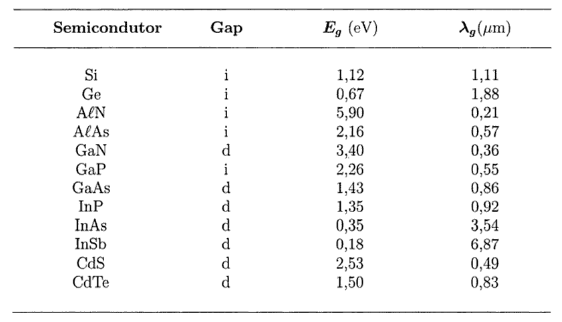
\includegraphics{figuras/semic.PNG}
    \end{center}
    \caption[Quadro de energias de gap e comprimentos de onda]{Quadro com os principais materiais semicondutores, tipo de banda, energia de gap e comprimento de onda resultante}
    \label{semicon}
\end{figure}

\subsection{Ergonomia da Iluminação}

A ergonomia é o estudo científico das relações homem e máquina no ambiente de trabalho, visando segurança e eficiência na interação entre estes. A norma regulamentadora que trata de ergonomia, a NR 17 \cite{norma}, traz orientações sobre luminosidade no ambiente de trabalho com o objetivo de proteger a saúde física e psicológica do trabalhador. Algumas das orientações da norma regulamentadora:

\begin{labeling}{17.5.3.3}
    \item[17.5.3] Em todos os locais de trabalho deve haver iluminação adequada, natural ou artificial, geral ou suplementar, apropriada à natureza da atividade.
    \item[17.5.3.1]  A iluminação geral deve ser uniformemente distribuída e difusa.
    \item[17.5.3.2] A iluminação geral ou suplementar deve ser projetada e instalada de forma a evitar ofuscamento, reflexos incômodos, sombras e contrastes excessivos.
    \item[17.5.3.3] Os níveis mínimos de iluminamento a serem observados nos locais de trabalho são os valores de iluminâncias estabelecidos na NBR 5413, norma brasileira registrada no INMETRO.
\end{labeling}

A NBR ISO/CIE 8995-1 \cite{normabr} substituiu a NBR 5413 e especifica condições de iluminação para ambientes de trabalho internos e visa a eficiência na execução de tarefas visuais com eficiência, conforto e segurança durante todo o tempo de trabalho, seja esta iluminação natural, artificial ou uma combinação de ambas. A fim de atingir esse objetivo vários critérios são levados em conta, entre eles estão: aspectos da cor da luz, cintilação e iluminância.

Esta legislação estabelece os valores de iluminâncias médias mínimas em serviço para iluminação artificial em interiores, onde se realizem atividades de comércio, indústria, ensino, esporte e outras. Estes valores estão condicionados a função do trabalhador e tempo de determinada tarefa. A iluminância é uma grandeza de luminosidade representada pela letra E, sua unidade de medida é o “lux”, para medí-la utiliza-se o luxímetro, e é definida como  "limite da razão do fluxo luminoso recebido pela superfície em torno de um ponto considerado, para a área da superfície quando esta tende para o zero." (NBR 8995-1, 2013).  A iluminância pode impactar em como uma pessoa percebe e realiza uma tarefa visual, de forma que altos valores de iluminância causam desconforto e ofuscamento e baixos valores tornam o ambiente de trabalho sem estímulo e tedioso.

%A cintilação e efeitos estroboscópicos são causado pelo chaveamento frequente ou oscilação da iluminância em função de aspectos elétricos da iluminação e pode provocar distração e efeitos fisiológicos como dores de cabeça. Podem ainda levar a situações de risco pela alteração da percepção de máquinas de rotação sincronizadas com a frequência de oscilação da iluminância. Este efeito é análogo ao de ver, em filmagens, a roda de um carro em movimento que parece estar girando devagar ou estar parada; o mesmo pode acontecer em uma fábrica com uma máquina síncrona iluminada por uma fonte de luz alimentada pela mesma rede elétrica que alimenta a máquina.%

\section{Internet das Coisas}

Ao longo da história, vários pensadores, cientistas e inventores fizeram previsões convergentes para o futuro, previsões de que um dia o mundo teria uma rede interconectada de computadores e sensores. Hoje vemos essas previsões tomarem forma e podemos vislumbrar esse futuro imaginado por grandes mentes do passado. Nikolas Tesla disse certa vez em uma entrevista em 1926: “... o planeta inteiro se tornará um cérebro gigante, o que significa que todas as coisas serão partes reais e harmônicas de um todo… e os instrumentos que nos permitirão realizar isso serão incrivelmente mais simples que os telefones atuais. Qualquer homem será capaz de carregar um seu próprio bolso”. Já o primeiro dispositivo cotidiano a se conectar a internet foi uma torradeira criada por John Romkey em 1990 e que se conectava a um computador pela pilha de protocolos TCP/IP (\acl{TCP} / \acl{IP}) podendo ser ligada ou desligada pela internet.

Tecnologias correlatas a \ac{IoT} vêm sendo adotadas, nos últimos anos, por empresas de todos os portes e abrindo espaço para novos empreendimentos. Não há restrições claras para os limites de aplicações para \ac{IoT}; aliada a outra importante tecnologia que vem sendo extensivamente explorada, a inteligência artificial, a \ac{IoT} consegue prover vantagens como aumento de produtividade, extrema versatilidade na obtenção de dados e redução de despesas. Um exemplo interessante é a aplicação de dispositivos conectados à rede na produção do leite \cite{milk} na qual produtores têm colocado sensores nos calcanhares, pescoço, mamas e intestino das vacas para prever com exatidão os ciclos férteis dos animais, medir a qualidade do leite antes de extraí-lo e monitorar a saúde da vaca.

\begin{figure}[ht]
    \begin{center}
    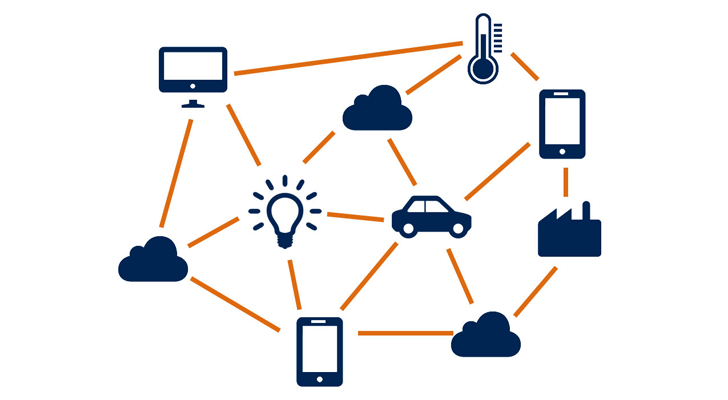
\includegraphics[width=0.7\textwidth]{figuras/iot}
    \end{center}
    \caption[Esquema dos elementos da Internet das Coisas.]{Esquema dos elementos da Internet das Coisas.}
    \label{iot}
\end{figure}

O mercado de \ac{IoT} pode ser separado em aplicações de consumo, da indústria e de serviços de infraestrutura da própria internet das coisas. O ramo voltado ao consumidor amplo é caracterizado principalmente por aplicações domiciliares como sistemas de segurança conectados e automação residencial, além de dispositivos vestíveis como monitores de sinais biológicos e relógios “inteligentes”. O setor industrial faz uso da internet das coisas em soluções de logística, agropecuária, sensoriamento em geral, planejamento urbano, monitoramento da rede elétrica, e vários outros exemplos. Para possibilitar que todos esse serviços de \ac{IoT} funcionem, há várias plataformas de infraestrutura de rede, sistemas embarcados, plataformas de software e serviços de armazenamento e análise de dados. Gigantes da tecnologia como “\textit{Google}”, “\textit{Microsoft}” e “\textit{Amazon}” têm setores totalmente voltado para \ac{IoT} e serviço de nuvem como o “\textit{Google Cloud}”, o “\textit{Microsoft Azure}” e o “\textit{Amazon Web Services}”.

\subsection{Redes de Computadores}

A comunhão dos computadores e das comunicações foi uma das principais revoluções tecnológicas modernas dando origem ao campo de redes de computadores com a demanda de organizar a comunicação entre computadores e criar sistemas computacionais para fazer essa comunicação.

Diz-se que uma rede de computadores é definida por dois ou mais computadores que, interligados por um meio físico, são capazes de trocar dados \cite{redes}. O conceito não especifica qual o meio físico que interliga os computadores que pode ser cabos metálicos, fibras óticas, micro-ondas, ondas de infravermelho; mas limita o meio a apenas um tipo, de forma que a “ampla rede mundial” (\textit{World Wide Web}) não é uma rede mas uma “rede de redes” e que a internet não é uma rede, e sim um sistema distribuído que, apesar de ser composto por vários computadores, é um sistema de softwares que opera sobre a rede e que dá a impressão ao usuário de ser um sistema coerente, uma rede não apresenta essa coerência aparente.

A \textit{World Wide Web} funciona de acordo com o modelo de cliente/servidor no qual um serviço cliente interage na rede por solicitações ao serviço servidor que responde a essas solicitações, podemos dizer também que o servidor provê recursos que os clientes consomem.

\subsection{A tecnologia \ac{WiFi}}

A popularização de computadores pessoais portáteis (notebooks) trouxe consigo a demanda que o acesso à internet se tornasse, também, móvel e assim foram desenvolvidas algumas arquiteturas de rede baseadas em ondas eletromagnéticas. A existência de diversos tipos de conexão sem fio (wireless) evidenciou a necessidade de uma padronização e assim o \ac{IEEE} lançou o padrão “802.11” para redes locais \cite{wifi} com uma série de especificação de controle de acesso ao meio (MAC) e camada física nas frequências de 900 MHz, 2.4, 3.6, 5 e 60 GHz com larguras de banda mais usuais de 20 ou 22 MHz e taxas de 1 até 3500 MB/s. Diversas revisões subsequentes do padrão como “a”, “b”, “g”, “n” especificam frequência, largura de banda, modulação entre outros fatores; a maioria dos dispositivos com internet sem fio é versátil para trabalhar com múltiplos modelos do padrão.

A \acf{WiFi} é uma marca da Wi-Fi Alliance, organização que promove a tecnologia e certifica produtos que obedecem a alguns requisitos de interoperabilidade do padrão \ac{IEEE} 802.11. Inicialmente, a variante do padrão 802.11 adotada pelo WiFi foi o "b" com taxas de transferência de até 11 MB/s, atualmente o padrão "g" vinha sendo usado e o padrão "n" começou a ser suportado desde 2009, com taxas de transferência de até 100 MB/s, todos estes operando na frequência de 2.4 GHz. A grande maioria dos roteadores WiFi comercializados hoje em dia suportam o padrão "802.11 b/g/n" com suporte às frequências de 2.4 e 5 GHz 

\section{\ac{MQTT}}

O \acf{MQTT} é um protocolo baseado em publicações e subscrições (ou assinaturas) de conectividade em rede para M2M (\textit{Machine to machine}) e \ac{IoT} construído sobre a camada subjacente de internet \ac{TCP}/\ac{IP}. Ele foi criado com o intuito de ser leve, simples e de fácil aplicação com o objetivo de conectar sensores em dutos de petróleo a satélites. A primeira versão do protocolo foi apresentada em 1999 por Andy Stanford-Clark da IBM e Arlen Nipper, e no final de 2014 se tornou um padrão aberto OASIS \cite{oasis} com suporte para diversas linguagens de programação.

O MQTT é um protocolo de transporte de mensagens com comunicação assíncrona o que torna possível desacoplar os usuários do sistema no espaço e no tempo, e viabiliza seu uso em situações com redes que não são confiáveis. Não obstante o protocolo apresenta codificação simples e quantidade mínima de dados de cabeçalho (informações além dos dados que se deseja transportar) em seus pacotes, características que implicam em uma alta eficiência de banda.

Como este protocolo funciona com o paradigma de publicações/subscrições para troca de mensagens entre as partes, ou clientes, e para isso ele apresenta um elemento mediador ao qual é dado nome \textit{broker}. Clientes que desejam enviar mensagens devem publicá-las em tópicos e clientes que querem receber mensagens de outros clientes devem subscrever os tópicos. O \textit{broker} tem o papel de conectar os clientes e mediar a troca de mensagens em tópicos. Em um sistema qualquer cliente pode subscrever qualquer tópico e publicar em qualquer tópico.

A estrutura do MQTT permite que os clientes sejam independentes no espaço, isto é, um cliente não precisa saber o endereço (IP ou porta) de outro para enviá-lo alguma mensagem; e torna-os independentes no tempo permitindo que o “ouvinte” não precise estar ativo quando alguma mensagem for enviada a ele.

\subsection{\textit{Broker} e Clientes}

Os elementos de uma rede baseada em MQTT baseada são, comumente, os clientes e um \textit{broker}. O broker funciona como um servidor que recebe as mensagens publicadas, classificadas por tópicos, e as encaminha para os clientes subscritos nos tópicos determinados. Clientes, por sua vez, são qualquer elemento que publique ou receba mensagens por subscrição podendo ser desde um sensor ou um atuador conectado, uma aplicação web que processa os dados, ou ainda um aplicativo móvel com poder de observar o comportamento dos sensores e publicar ações para os atuadores.

\subsection{Publicações e Subscrições}

O paradigma de comunicação por publicações e subscrições (ou simplesmente “\textit{PubSub}”) é um paradigma no qual remetentes, chamados de publicadores, não especificam quais serão os destinatários, chamados de subscritores, das mensagens enviadas; em vez disso as mensagens são classificadas por assuntos, chamados de tópicos, assim um cliente que publica uma mensagem não controla quais clientes a receberam ou, ainda, se será recebida por qualquer cliente. Consequentemente, clientes que subscrevem determinados tópicos não, necessariamente, sabem qual cliente originou determinada mensagem apesar de tópicos estarem comumente atrelados a publicadores, isso significa que comumente um tópico têm mensagens publicadas por um único publicador.

Tópicos são representados por “\textit{strings}” organizadas de forma hierárquica por níveis os quais são separados por barras (“/”) lembrando o padrão URI de endereços. Os tópicos permitem filtrar mensagens por categorias, clientes ou tipo de dados. Isto significa que o sistema de automação de uma casa com vários sensores de temperatura e umidade pode ter alguns de seus tópicos nomeados da seguinte forma:

\begin{center}
    \texttt{“home/jardim/sensor1/temperatura”}
    
    \texttt{“home/jardim/sensor3/umidade”}
\end{center}

O sistema de tópicos apresenta ainda flexibilidade no que diz respeito ao acesso generalizado a mensagens. Usando o exemplo anterior, caso um cliente deseje subscrever todos os tópicos referentes a temperatura, ele pode usar caracteres “coringa” como “+” ou “\#” da seguinte forma:

\begin{center}
    \texttt{“home/+/+/temperatura”}
    
    \texttt{“home/\#/\#/temperatura”}
\end{center}

\begin{figure}[ht]
    \begin{center}
    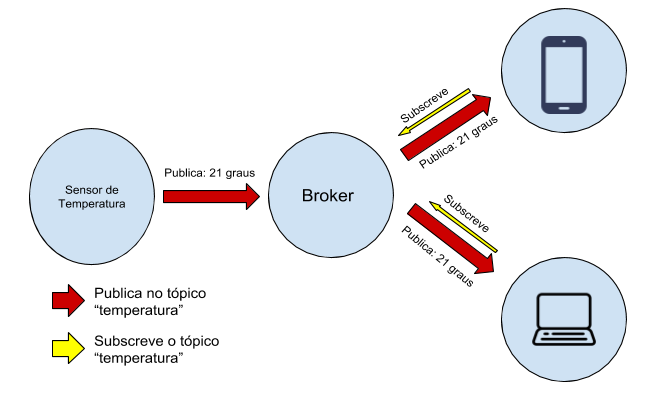
\includegraphics[width=0.7\textwidth]{figuras/mqtt.PNG}
    \end{center}
    \caption[Ilustração do funcionamento do protocolo MQTT.]{Ilustração do funcionamento do protocolo MQTT com três clientes e o broker trocando mensagens pelo tópico "temperatura".}
    \label{mqtt}
\end{figure}

A troca de mensagens funciona da seguinte forma:
\begin{itemize}
    \item[1 -] O cliente conecta-se ao \textit{broker} por meio de uma conexão TCP/IP e pode assinar (ou subscrever) qualquer tópico de mensagens do \textit{broker}.
    \item[2 -] O cliente pode publicar mensagens ao enviar o tópico e o conteúdo da mensagem (também chamado de \textit{payload}) ao \textit{broker}.
    \item[3 -] O broker encaminha as mensagens publicadas aos clientes.
\end{itemize}

\subsection{QoS}

Qualidade de serviço (\acl{QoS}) é uma padronização das capacidades de troca de dados em uma rede que determina fatores como a previsibilidade, retardo e a qualidade geral da comunicação; mais especificamente no caso do protocolo MQTT, os níveis de qualidade de serviço (0, 1 e 2) são uma espécie de “acordo” entre o transmissor e o receptor da mensagem quanto a garantia de entrega de uma mensagem, e isso impacta diretamente a previsibilidade da comunicação.

Os três níveis de QoS no MQTT são:
\begin{itemize}
    \item[0 -] Não há garantia de entrega.
    \item[1 -] Mensagem é entregue pelo menos uma vez (pode ser mais).
    \item[2 -] A mensagem é entregue exatamente uma vez.
\end{itemize}

A garantia de entrega dos níveis 1 e 2 é devido a confirmações de recebimento e reenvio em caso de falha. O nível 0 não inclui confirmações de entrega ou reenvios, é comumente chamado de nível de melhor esforço possível ou “\textit{fire and forget}” (atire e esqueça); apesar de ser o nível de pior previsibilidade, apresenta também a menor latência de comunicação.

Ao usar o nível de QoS 1, um cliente que envia uma mensagem ao broker, ou o inverso, contará com a garantia que essa mensagem será entregue pelo menos uma vez, mas pode ser mais de uma vez. Uma mensagem publicada pelo cliente será armazenada por ele até que receba uma confirmação, um “\textit{puback}” (confirmação de publicação), com a mesma identificação da mensagem enviada. Caso não receba a confirmação até determinado tempo (“\textit{ack timeout}”) a mensagem será reenviada com, com informação que está duplicada, periodicamente até o recebimento do “\textit{puback}”.

O nível mais alto de QoS, 2, é o que provê mais previsibilidade e envolve a maior quantidade de troca de informações na troca de uma mensagem. Esse nível apresenta confirmação de recebimento e confirmação de recebimento da confirmação. A maioria de serviços de MQTT baratos ou grátis, para testes e "hobbistas", não dão suporte ao QoS de nível 2.

\section{Sistemas Embarcados}

Uma definição sucinta de sistema é um conjunto de processos ou mesmo sistemas conectados que realizam uma ou mais tarefas como um todo. Como o nome sugere um sistema embarcado é um sistema eletrônico que faz parte de um sistema maior com a função de, muitas vezes, controlar, interfacear, observar outros sistemas eletrônicos ou não. É um programa computacional, ou \textit{software}, que é executado por um sistema físico, o \textit{hardware}, de capacidades adequadas ou projetadas para a tarefa a ser executada, diferente de computadores pessoais, de propósito geral, que possuem capacidade de executar uma grande variedade de tarefas à demanda do usuário.

Os sistemas embarcados são parte de fundamental da maioria dos sistemas eletrônicos usados atualmente por apresentar padronização de comunicação entre estas unidades, facilidade e simplicidade de processamento de sinais e consumo de energia otimizado. Uma característica importante de sistemas embarcados é que existem arquiteturas dos mais variados tipos, que são especificados para executar os mais variados tipos de tarefas: desde arquiteturas que suportam sistemas operacionais complexos para processamento de imagens em tempo real, até arquiteturas simples com poucos transistores e outros componentes que realizam tarefas como ligar uma lâmpada ou contar tempo.

\subsection{Microcontroladores}

Microcontroladores são sistemas embarcados cuja função é a de controlar o sistema do qual fazem parte. Dentro da classe de sistemas dedicados estão os microcontroladores que são compostos, em geral, por uma unidade central de processamento (CPU), memória não-volátil para dados e instruções, memória volátil de acesso aleatório (RAM), oscilador e periféricos que geram entradas ou recebem saídas do processador como contadores, \textit{timers}, módulos de comunicação seriais e paralelos, conversores analógicos e digitais . Microcontroladores estão presentes em quase todos equipamentos eletrônicos que se possa imaginar: a indústria de eletrônica de consumo e a indústria automobilística fazem uso extensivo de microcontroladores.

\begin{figure}[ht]
    \begin{center}
    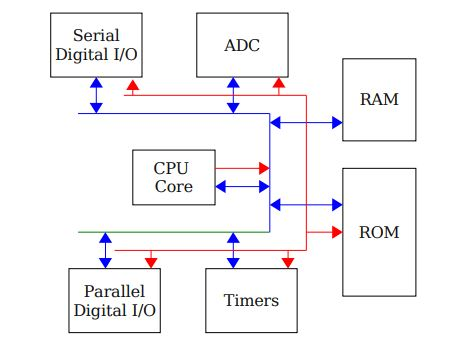
\includegraphics[width=0.4\textwidth]{figuras/micro.JPG}
    \end{center}
    \caption[Diagrama de blocos de um microcontrolador.]{Diagrama de blocos de um microcontrolador com o núcleo de processamento e seus diversos periféricos}
    \label{micro}
\end{figure}

\subsection{ESP-8266}

O ESP-8266 \cite{esp} é um \acf{SoC} com capacidade de comunicação \ac{WiFi} padrão 802.11 b/g/n da fabricante chinesa \textit{Espressif}. Conta com uma CPU de 32 bits RISC (\textit{Reduced Instronction Set Computer}), o \textit{Xtensa} LX106 da \textit{Cadence Tensilica} de baixa potência (menos de 1 mW em \textit{standby}), possui \textit{clock} de 80 MHz, uma ROM de \textit{boot} de 64KB, uma RAM de instruções de 64 KB e uma RAM para dados de 96 KB. Possui a pilha TCP/IP já integrada. Sua tensão de alimentação recomendada é de 3.3V.

\begin{figure}[ht]
    \begin{center}
    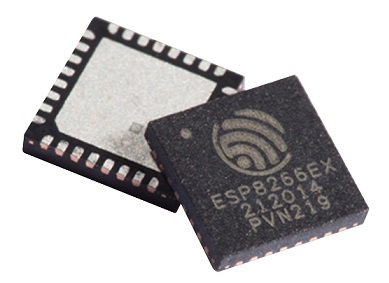
\includegraphics[width=0.3\textwidth]{figuras/esp8266.jpg}
    \end{center}
    \caption[ESP-8266 em seu encapsulamento QFN.]{Ilustração do circuito integrado ESP-8266 em seu encapsulamento QFN.}
    \label{esp8266}
\end{figure}

O ESP8266 possui interfaces "UART", "I2C" (apenas a função de mestre implementada em suas bibliotecas de desenvolvimento de \textit{software} oficial, mas há implementações para escravo I2C da comunidade), "SPI" (com três pinos de \textit{device enable} além dos outros pinos usuais do protocolo). Possui 16 pinos de uso geral podendo ser configurados com pull-up/down internos, interrupção por nível ou borda em seus pinos de entrada e saída, opção configurável de saída open-drain ou push-pull, ou ainda saída analógica de PWM com resolução de 10 bits em qualquer pino e uma entrada analógica (ADC). Seus pinos possuem proteção contra sobrevoltagem de até 5,8 V e conseguem fornecer até 12 mA de corrente cada um.

\begin{figure}[ht]
    \begin{center}
    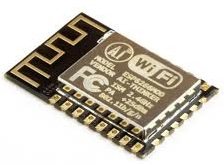
\includegraphics[width=0.3\textwidth]{figuras/esp12.jpg}
    \end{center}
    \caption[Kit de desenvolvimento ESP-12.]{Ilustração kit de desenvolvimento ESP-12 baseado no ESP-8266}
    \label{esp12}
\end{figure}

A \textit{Espressif} comercializa diferentes módulos baseados no ESP8266, numerados de 1 até 12, que facilitam o desenvolvimento e a produção de produtos por já integrar circuitos ou chips de antena, sistema de alimentação e outros circuitos com o seu SoC. O ESP-01, por exemplo, possui apenas oito pinos, sendo dois deles "VCC" e "GND", e foi desenvolvido para ser usado como um simples modulo WiFi-serial. O ESP-12F possui os 16 GPIOs disponíveis e uma memória flash externa de 4MB "SPI". Esse módulo é usado na maioria das plataformas de desenvolvimento do ESP-8266, como o “\textit{NodeMCU}” e o “\textit{Wemos D1 Mini}”. Estas plataformas possuem recursos que facilitam o desenvolvimento como interface USB-serial, botão de \textit{reset} e conectores apropriados para \textit{protoboards}.
